\documentclass[rc]{physicsinprogress}

\pipvolume{2}
\pipissuedate{Feb. 2026}

\usepackage{siunitx}

\begin{document} 


\title{It takes two: finding the normal modes in a coupled pendulum system}
\author{Brookelyn H Velmont}
\affiliation{%
Department of Physics and Astronomy,  Carthage College, 2001 Alford Park Drive, Kenosha, WI 53140, USA
}%
\collaboration{Received January 29, 2026, Published online February 5, 2026}
\begin{abstract}
 The normal modes of a system of two coupled pendulums were determined by using angular displacement data recorded with rotary motion sensors. As the pendulums oscillated, the angular displacements $\theta_1(t)$ and $\theta_2(t)$ were measured simultaneously and used to construct a covariance matrix describing their correlated motion. Diagonalization of this covariance matrix revealed two independent mode coordinates corresponding to in-phase and out-of-phase oscillations. Projection of the experimental data onto these mode coordinates produced a clear separation of the system's behaviors, with the in-phase mode dominating the motion.
\end{abstract}

\maketitle

\vspace*{\fill}
\section{Introduction}
Synchronization is one of the most common phenomena observed in nature, yet the physical mechanisms underlying such behavior in non-linear systems are still an active area of study. Christiaan Huygens played a key role in the early mathematical understanding of pendular motion through his development of the first pendulum clock. While the motion of a single pendulum is well described by simple harmonic motion at small angles, many real physical systems often involve multiple oscillators that exchange energy. Huygens observed that when he hung two pendulums from a common support, it took about a half an hour for them to gradually synchronize, oscillating out of phase at the same frequency. He referred to this as “the sympathy of two clocks” \cite{Pena_Ramirez_undated-ie}. When two pendulums are coupled in this manner, their behaviors become interdependent, leading to collective behavior that cannot be explained when analyzing each pendulum individually \cite{pena2016sympathy}.

A defining feature of coupled pendulum systems is the existence of normal modes, which are specific patterns of motion in which the pendulums oscillate at a single characteristic frequency with a fixed phase relationship. For two coupled pendulums, these modes correspond to in-phase and out-of-phase oscillations, each with distinct frequency determined by the coupling strength and the physical parameters of the system \cite{smith2003two}. By measuring the angular displacement of each pendulum as a function of time, the normal modes can be identified and analyzed. The coupled pendulum system thus serves as a foundational example for studying normal modes, synchronization, and energy transfer in more complex physical systems.
\vspace{\fill}
\vspace{\fill}
\section{Key Findings}
This experiment consisted of two PASCO CI-6538 Rotary Motion Sensors  mounted on a rigid point as seen in Fig.\ref{fig:pic}. These sensors consisted of rods of negligible mass, each with a point mass fixed at the bottom of the rod. The two pendulums are connected in the center of the rods via a light spring. This connection allows for an energy transfer during oscillation. One pendulum was kept at the equilibrium position while the other was displaced by $\theta_1$ and released from rest. Angular displacement was measured over 30-second intervals while the pendulums swung in beat. Data for ten runs were collected. Run 9 was chosen for the analysis because it had the greatest ratio of eigenvalues, indicating strong separation between the normal modes and minimal modal mixing. 

\begin{figure}
    \centering
    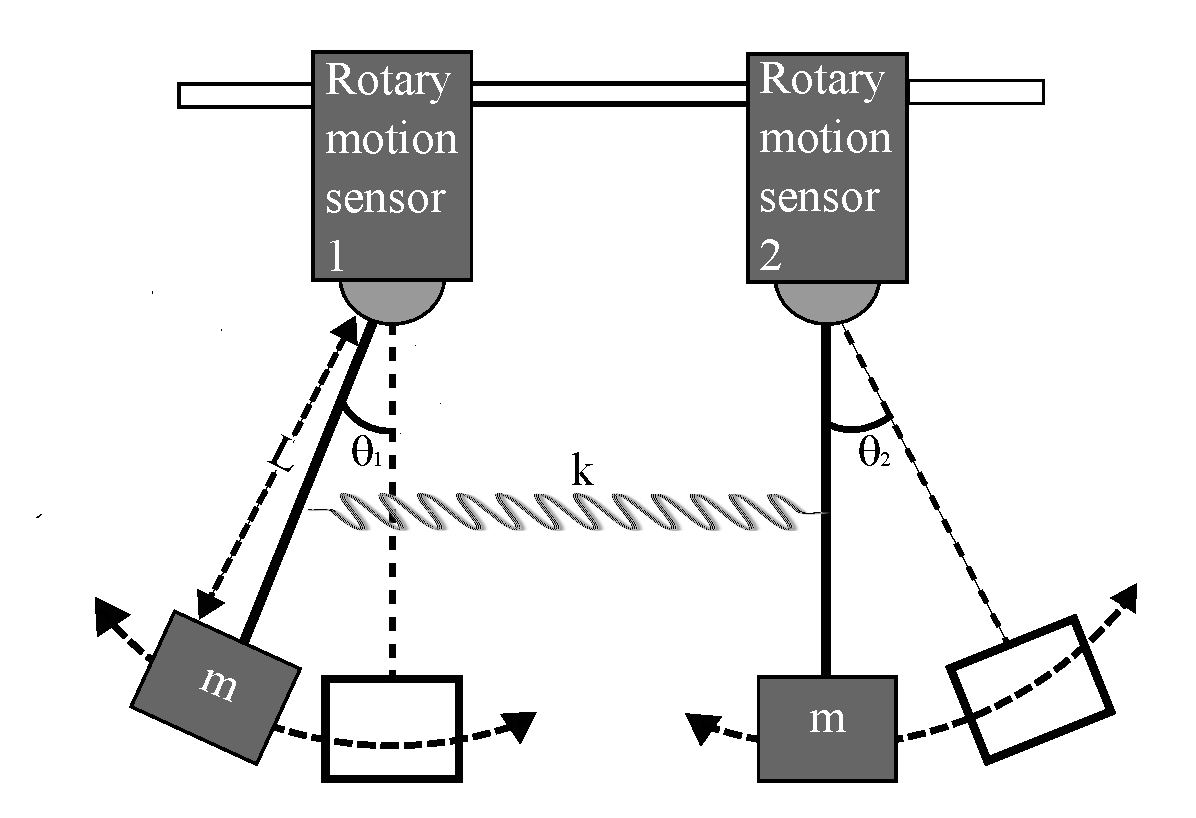
\includegraphics[ width=0.9\linewidth] {coupledosc.pdf}
    \caption{A schematic of the coupled pendulums used in this experiment, consisting of two rotary motion sensors made up of massless rods with point masses at the bottom of each, the pendulums attached with a light spring.}
    \label{fig:pic}
\end{figure}

The goal of the experiment is to identify the normal modes of the coupled pendulum. Normal modes are the characteristic patterns of motion in which the pendulums oscillate at a single frequency with a fixed phase relationship. To do this, the measured angular displacements, $\theta_1(t)$ and $\theta_2(t)$, were first centered by subtracting the mean value for each pendulum. To quantify correlations between the two pendulums, the covariance matrix is constructed. Its elements are defined by 
\begin{align}
A_{11} &= \left\langle (\theta_1 - \bar{\theta}_1)^2 \right\rangle, \\
A_{22} &= \left\langle (\theta_2 - \bar{\theta}_2)^2 \right\rangle, \\
A_{12} &= \left\langle (\theta_1 - \bar{\theta}_1)(\theta_2 - \bar{\theta}_2) \right\rangle,
\end{align}
where $\langle \cdot \rangle$ denotes a time average over the dataset.

The resulting covariance matrix is 
\begin{equation}
\mathbf{A} =
\begin{pmatrix}
A_{11} & A_{12} \\
A_{12} & A_{22}
\end{pmatrix}.
\end{equation}

The normal modes of the coupled system correspond to the eigen vectors of the covariance matrix. The eigenvalues $\lambda$ are obtained by solving the characteristic equation 
\begin{equation}
\det(\mathbf{A} - \lambda \mathbf{I}) = 0,
\end{equation}
which yields
\begin{equation}
\lambda_{1,2} =
\frac{(A_{11} + A_{22}) \pm
\sqrt{(A_{11} + A_{22})^2 - 4(A_{11}A_{22} - A_{12}^2)}}{2}.
\end{equation}

The larger eigenvalue corresponds to the dominant mode of motion.

For each eigenvalue $\lambda_k$, the corresponding eigenvector $\mathbf{x}^{(k)}$ satisfies
\begin{equation}
(\mathbf{A} - \lambda_k \mathbf{I})\mathbf{x}^{(k)} = 0.
\end{equation}
Solving this system yields eigenvectors of the form
\begin{equation}
\mathbf{x}^{(k)} =
\begin{pmatrix}
\dfrac{A_{12}}{\lambda_k - A_{11}} \\
1
\end{pmatrix},
\end{equation}
which are normalized such that
\begin{equation}
\left\lVert \mathbf{x}^{(k)} \right\rVert = 1.
\end{equation} 

These eigenvectors represent the relative amplitudes of the two pendulums on each normal mode. The normal mode coordinates are obtained by projecting the angular displacement onto the eigenvectors: 
\begin{align}
\eta_1(t) &= x_1^{(1)}\theta_1(t) + x_2^{(1)}\theta_2(t), \\
\eta_2(t) &= x_1^{(2)}\theta_1(t) + x_2^{(2)}\theta_2(t).
\end{align}

The resulting time series $\eta_1(t)$ and $\eta_2(t)$ correspond to the in-phase and out-of-phase normal modes of the coupled pendulum system.

Using the angular displacement data from a representative experimental run, the covariance matrix was found to be
\begin{equation}
\mathbf{A} =
\begin{pmatrix}
0.00944 & 0.00616 \\
0.00616 & 0.01002
\end{pmatrix},
\end{equation}
where all entries are given in units of rad$^2$.

\begin{figure}
    \centering
    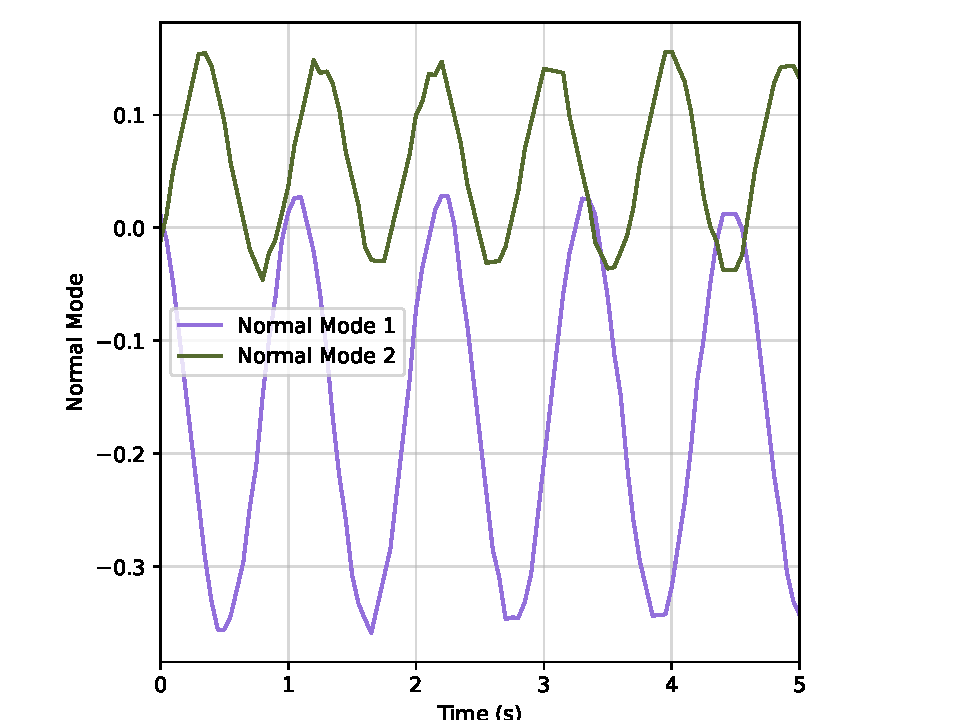
\includegraphics[ width=1\linewidth] {normalmodes.pdf}
    \caption{Plot of normal modes 1\&2 as a function of time. The in-phase mode (Normal Mode 1, bottom wave) dominates the motion, while the out-of-phase mode (Normal Mode 2, top wave) exhibits a smaller amplitude, consistent with the relative magnitudes of the covariance matrix eigenvalues.}
    \label{fig:normal}
\end{figure}

Diagonalization of the covariance matrix yielded eigenvalues
\begin{equation}
\lambda_1 = 0.01590, \qquad \lambda_2 = 0.00356,
\end{equation}
with corresponding normalized eigenvectors
\begin{equation}
\mathbf{x}^{(1)} =
\begin{pmatrix}
0.690 \\
0.724
\end{pmatrix},
\qquad
\mathbf{x}^{(2)} =
\begin{pmatrix}
-0.724 \\
0.690
\end{pmatrix}.
\end{equation}

The normal mode coordinates were constructed by projecting the angular displacements onto the eigenvectors,
\begin{align}
\eta_1(t) &= 0.690\,\theta_1(t) + 0.724\,\theta_2(t), \\
\eta_2(t) &= -0.724\,\theta_1(t) + 0.690\,\theta_2(t).
\end{align}
 
\section{Conclusion}
The first eigenvector has components of the same sign, indicating an in-phase mode in which both pendulums oscillate together. The second eigenvector has components of opposite sign, corresponding to an out-of-phase mode where the pendulums oscillate in opposition.

Fig.\ref{fig:normal}. shows the time evolution of the two normal mode coordinates obtained from the angular displacement data. The motion is clearly decomposed into an in-phase component and an out-of-phase component, indicating that the coupled pendulum system is well described by two independent normal modes.

Normal Mode 1 exhibits a significantly larger amplitude than Normal Mode 2, consistent with the larger associated eigenvalue of the covariance matrix. This indicates that the majority of the system’s variance, and therefore the dominant motion, is contained in the in-phase mode. Physically, this corresponds to both pendulums oscillating together with similar amplitudes, suggesting that this mode is more easily excited by the initial conditions of the system.

Normal Mode 2 displays a smaller-amplitude oscillation and corresponds to out-of-phase motion of the pendulums. The reduced amplitude of this mode suggests weaker excitation, which may arise from asymmetries in the initial displacement or from dissipative effects that preferentially damp higher-energy relative motion between the pendulums.

The clean separation of the motion into two distinct mode coordinates demonstrates that the covariance matrix diagonalization effectively isolates the system’s normal modes and confirms the expected behavior of a weakly coupled two-oscillator system.

The coupled pendulum system exhibits behaviors that are well captured by two independent normal modes corresponding to collective and relative motion. The successful extraction of these modes from experimental data demonstrates how normal mode behavior emerges naturally in real, imperfect systems and highlights covariance-based methods as a powerful tool for analyzing coupled oscillations.

While the covariance matrix method effectively isolates the normal modes, it is important to acknowledge sources of experimental error. Random fluctuations in the rotary sensor readings, finite sampling over 30-second intervals, and slight deviations from the ideal pendulum model introduce uncertainties in the measured eigenvalues and eigenvectors. Additionally, small damping effects may reduce the amplitude of the out-of-phase mode relative to the in-phase mode. Despite these limitations, the overall mode structure is clearly observed and consistent across multiple runs, indicating that the method is robust for identifying normal modes in real coupled systems.

Understanding the normal modes of coupled pendulums also has practical relevance in engineering and physics. For example, analyzing vibrations in bridges, mechanical structures, or coupled oscillatory circuits often relies on identifying independent modes to predict and control system behavior, illustrating the broader applicability of these experimental and analytical techniques.

\section*{acknowledgments}
This research would not have been made possible without funding from the Carthage College Physics and Astronomy Department along with assistance from Dr. Joseph Anderson.

\vspace{\fill}

\section*{Data Availability Statement}
A Jupyter notebook containing all the experimental data, data analysis, figure generation, and additional information on uncertainty analysis can be found in the supplemental materials. \footnote{See online article posting for access to supplemental material.}


\bibliography{bib.bib}

\end{document}
